% ============================================================
%  04_csdl.tex – Chương 4: Thiết kế dữ liệu
% ============================================================
\chapter{Thiết Kế Dữ Liệu}

\section{Tổng Quan}

Hệ thống sử dụng PostgreSQL 15. Phần lớn bảng thương mại điện tử được Medusa quản lý thông qua module và migration; dự án bổ sung các bảng riêng cho nội dung website, phân quyền, nguyên liệu và yêu cầu mua số lượng lớn. Vì Medusa khuyến khích cô lập mô-đun, quan hệ giữa mô-đun lõi và mô-đun tùy biến được khai báo bằng module link.

Ngoài cơ sở dữ liệu quan hệ, hệ thống còn dùng Redis cho dữ liệu tạm thời, Meilisearch cho chỉ mục tìm kiếm và MinIO cho tệp nhị phân. Ba thành phần này không thay thế PostgreSQL mà phục vụ các kiểu truy cập chuyên biệt.

\section{Nhóm Thực Thể Lõi Của Medusa}

\begin{longtable}{@{}p{0.22\textwidth} p{0.28\textwidth} p{0.42\textwidth}@{}}
  \toprule
  \textbf{Miền} & \textbf{Thực thể tiêu biểu} & \textbf{Ý nghĩa} \\
  \midrule
  \endhead
  Catalog & Product, ProductVariant, ProductCategory, ProductImage & Thông tin sản phẩm, biến thể, danh mục và ảnh. \\
  Giá bán & Price, PriceSet, Region & Giá theo biến thể, tiền tệ và khu vực bán hàng. \\
  Kho & InventoryItem, InventoryLevel, StockLocation & Số lượng hàng hoặc nguyên liệu tại từng vị trí kho. \\
  Khách hàng & Customer, AuthIdentity & Hồ sơ khách và định danh đăng nhập. \\
  Đơn hàng & Order, OrderItem, OrderAddress & Đơn, dòng hàng, địa chỉ và metadata vận hành. \\
  Khuyến mãi & Promotion, ApplicationMethod, Campaign & Mã giảm giá, cách tính và giới hạn chương trình. \\
  Quản trị & User, AuthIdentity & Người dùng nội bộ và thông tin xác thực. \\
  \bottomrule
\end{longtable}

\section{Các Model Tùy Biến}

\subsection{Mô-đun Site}

\begin{longtable}{@{}p{0.23\textwidth} p{0.31\textwidth} p{0.38\textwidth}@{}}
  \toprule
  \textbf{Model} & \textbf{Thuộc tính chính} & \textbf{Mục đích} \\
  \midrule
  \endhead
  \texttt{site\_banner} & title, subtitle, image, link, order, active & Banner động trên frontend, có thứ tự và trạng thái. \\
  \texttt{site\_setting} & key, value (JSON) & Cấu hình tổng quát như giao hàng, chính sách, hotline và chatbot. \\
  \shortstack[l]{\texttt{site\_blog\_}\\\texttt{category}} & name, slug, description & Danh mục bài viết. \\
  \texttt{site\_blog\_post} & title, slug, excerpt, content, image, author, category, published, published\_at & Nội dung blog và trạng thái xuất bản. \\
  \shortstack[l]{\texttt{site\_contact\_}\\\texttt{message}} & name, email, phone, message, status & Yêu cầu liên hệ từ khách hàng. \\
  \shortstack[l]{\texttt{site\_chatbot\_}\\\texttt{question\_log}} & message, normalized\_message, response\_mode, resolved, metadata & Theo dõi chất lượng câu trả lời chatbot. \\
  \bottomrule
\end{longtable}

\subsection{Mô-đun RBAC}

\begin{longtable}{@{}p{0.22\textwidth} p{0.33\textwidth} p{0.37\textwidth}@{}}
  \toprule
  \textbf{Model} & \textbf{Thuộc tính chính} & \textbf{Mục đích} \\
  \midrule
  \endhead
  \texttt{role} & name, description, guard\_name, is\_default, permissions (JSON) & Nhóm quyền của người dùng quản trị. \\
  \texttt{permission} & name, description, guard\_name & Quyền nguyên tử dạng \texttt{module.action}. \\
  \bottomrule
\end{longtable}

Danh sách ID role hiện được lưu trong metadata của User và đồng thời dự án có module link User--Role. Mỗi role lưu mảng ID permission trong trường JSON. Cách này linh hoạt khi seed dữ liệu nhưng cần chuẩn hóa để tránh hai nguồn liên kết cùng tồn tại lâu dài.

\subsection{Mô-đun Ingredients}

\begin{longtable}{@{}p{0.22\textwidth} p{0.33\textwidth} p{0.37\textwidth}@{}}
  \toprule
  \textbf{Model} & \textbf{Thuộc tính chính} & \textbf{Mục đích} \\
  \midrule
  \endhead
  \texttt{ingredient} & name, type, unit, cost\_price & Nguyên liệu như trái cây, sốt, sữa chua hoặc thành phần khác. \\
  \texttt{recipe\_item} & variant\_id, quantity, ingredient & Định mức một nguyên liệu cho một biến thể sản phẩm. \\
  \bottomrule
\end{longtable}

Một Ingredient liên kết một-một với InventoryItem của Medusa. Khi đặt $q$ sản phẩm, lượng nguyên liệu $i$ cần dùng được tính theo:

\begin{equation}
  D_i = \sum_{v \in V} q_v \times r_{v,i}
\end{equation}

trong đó $q_v$ là số lượng biến thể $v$ trong đơn và $r_{v,i}$ là định mức nguyên liệu $i$ trong công thức của biến thể đó. Đơn chỉ được tạo khi tồn khả dụng của mọi nguyên liệu không nhỏ hơn $D_i$.

\subsection{Các mô-đun khác}

\begin{itemize}[leftmargin=2em, itemsep=4pt]
  \item \texttt{bulk\_order}: lưu tên công ty, email, điện thoại, ngày yêu cầu, ghi chú và trạng thái của đơn số lượng lớn.
\end{itemize}

\section{Quan Hệ Dữ Liệu}

\begin{diagramcanvas}
\begin{figure}[H]
  \centering
  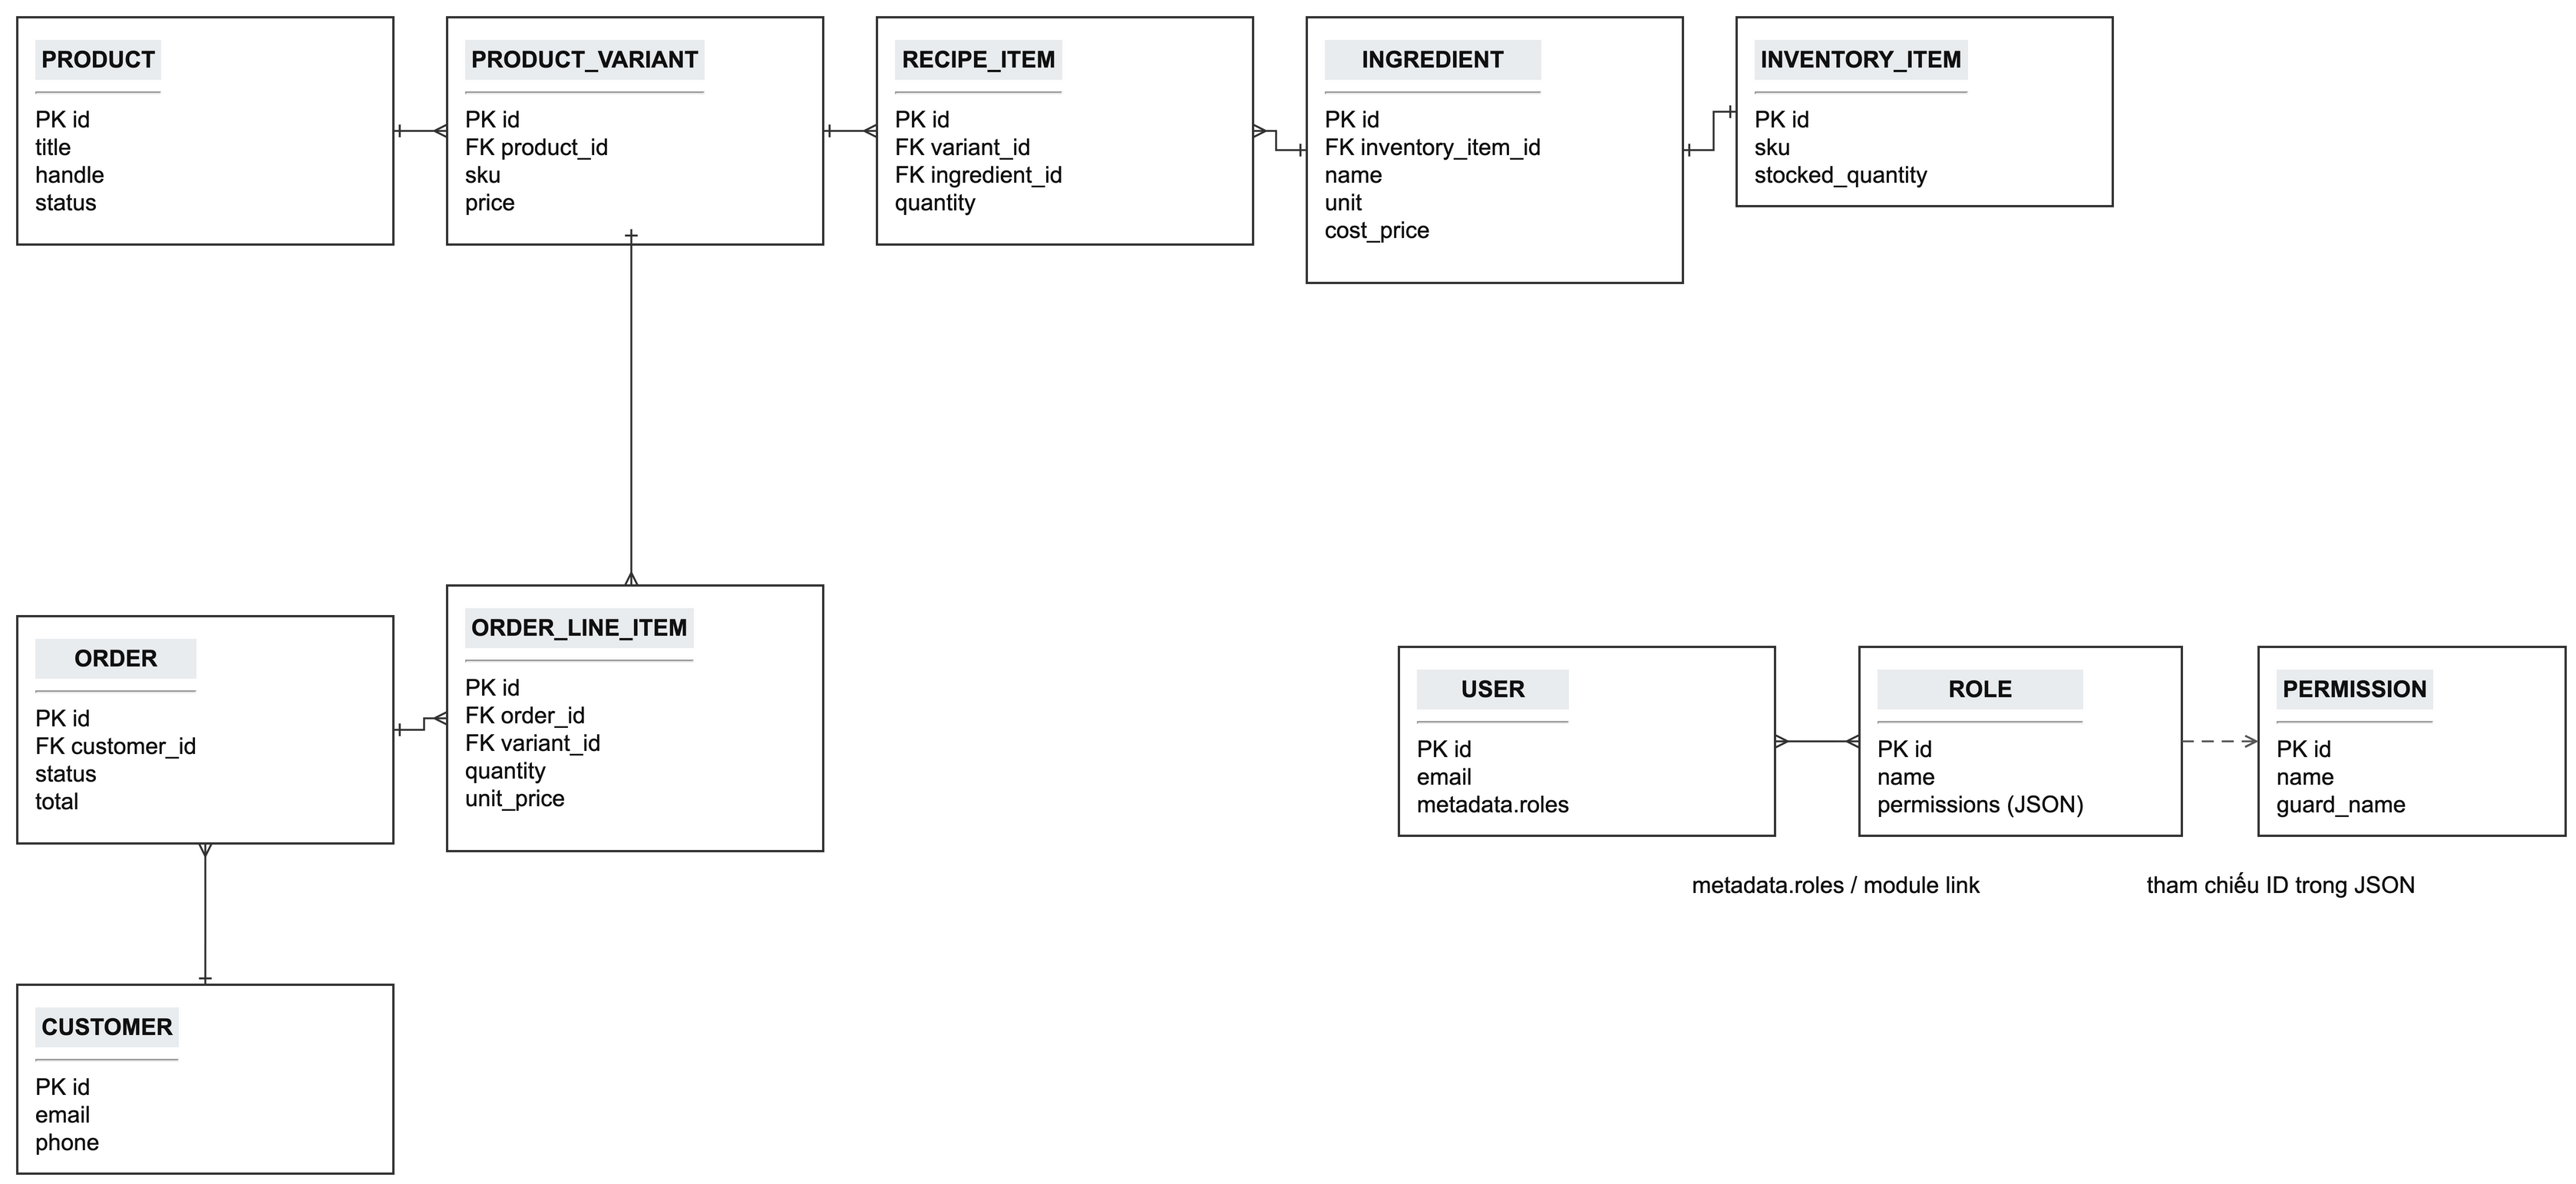
\includegraphics[width=\linewidth,height=0.52\textheight,keepaspectratio]{images/erd.drawio.png}
  \caption{ERD logic của các thực thể nghiệp vụ chính}
  \label{fig:data-links}
\end{figure}
\end{diagramcanvas}

BlogCategory có quan hệ một-nhiều với BlogPost. User liên kết Role; Role tham chiếu Permission. Ingredient liên kết InventoryItem, còn RecipeItem nối biến thể với Ingredient.

\section{Ánh Xạ Mô Hình Miền Sang Lưu Trữ}

ERD chỉ trình bày các bảng quan trọng để giữ khả năng đọc. Trong triển khai thực tế, Medusa tách giá, kho, địa chỉ và liên kết module thành nhiều bảng chuyên biệt. Product--ProductVariant và Order--OrderLineItem là các quan hệ sở hữu; RecipeItem là thực thể kết hợp mang thuộc tính \texttt{quantity}; RBAC đi qua module link hoặc bảng liên kết thay vì làm rò rỉ model của module lõi vào module tùy biến.

Các khóa nghiệp vụ cần ràng buộc duy nhất gồm handle sản phẩm, SKU biến thể, email đăng nhập và tên quyền trong cùng guard. Khóa ngoại hoặc module link thường dùng để lọc cần có index, nhất là các liên kết từ order tới customer và từ recipe item tới variant/ingredient. Truy vấn danh sách cần index kết hợp theo trạng thái và thời gian tạo thay vì tải toàn bộ bản ghi rồi lọc tại ứng dụng.

Lược đồ hiện tại tập trung vào catalog, order, RBAC, site content, ingredient và inventory. Các bảng không còn phục vụ chức năng hiện hành không được đưa vào ERD để sơ đồ gọn và đúng với mã nguồn mới nhất.

\section{Nhất Quán Giao Dịch}

Checkout chạm tới nhiều loại dữ liệu: giá và catalog, số lượng nguyên liệu, promotion, order và event hậu xử lý. PostgreSQL nên bao phủ phần ghi giao dịch cốt lõi; các tác vụ ngoài giao dịch như cập nhật Meilisearch hoặc gửi email nên đi qua event/outbox và có retry. Khóa idempotency phải gắn với kết quả tạo đơn để cùng một request lặp lại trả về cùng order thay vì trừ tồn hai lần. Với tồn kho cạnh tranh, bước giữ hoặc trừ hàng cần khóa/điều kiện cập nhật nguyên tử, không chỉ đọc số lượng rồi ghi lại.

\section{Dữ Liệu Phi Quan Hệ}

\subsection{Redis}

Redis lưu cache có TTL, rate-limit counter và giỏ hàng phiên. Trong development, Redis có thể tắt bằng cấu hình; hệ thống sử dụng implementation giả hoặc localStorage để giảm phụ thuộc. Trong production, Redis cũng có thể làm event bus nhằm xử lý subscriber ngoài tiến trình request.

\subsection{Meilisearch}

Mỗi tài liệu tìm kiếm được suy ra từ Product và các quan hệ liên quan. Các trường được tìm kiếm gồm title, description, slug và tên danh mục; trường lọc gồm trạng thái, category và price range; trường sort gồm thời gian và giá. PostgreSQL vẫn là nguồn dữ liệu chuẩn, còn Meilisearch là bản sao tối ưu truy vấn.

\subsection{MinIO}

MinIO cung cấp API tương thích S3. Cơ sở dữ liệu chỉ lưu object key hoặc URL; dữ liệu nhị phân được lưu trong bucket \texttt{mong-media}. API media quản trị chịu trách nhiệm upload, liệt kê và xóa object.

\section{Toàn Vẹn, Sao Lưu và Bảo Mật Dữ Liệu}

\enlargethispage{2\baselineskip}
\begin{itemize}[leftmargin=2em, itemsep=4pt]
  \item Migration của từng mô-đun phải được áp dụng đồng bộ với phiên bản mã nguồn.
  \item PostgreSQL và bucket MinIO cần được sao lưu; chỉ mục Meilisearch có thể dựng lại từ catalog.
  \item Secret kết nối, khóa Groq, Meilisearch master key và thông tin MinIO không được dùng giá trị mặc định ở production.
  \item API không trả dữ liệu cá nhân cho chatbot; lịch sử đơn được lọc theo customer ID từ token.
  \item Checkout nhiều bước cần workflow có giao dịch và hoàn tác để bảo đảm tính nguyên tử.
\end{itemize}
